%%%%%%%%%%%%%%%%%%%%%%%%%%%%%%%%%%%%%%%%%
% baposter Portrait Poster
% LaTeX Template
% Version 1.0 (15/5/13)
%
% Created by:
% Brian Amberg (baposter@brian-amberg.de)
%
% This template has been downloaded from:
% http://www.LaTeXTemplates.com
%
% License:
% CC BY-NC-SA 3.0 (http://creativecommons.org/licenses/by-nc-sa/3.0/)
%
%%%%%%%%%%%%%%%%%%%%%%%%%%%%%%%%%%%%%%%%%

%----------------------------------------------------------------------------------------
%	PACKAGES AND OTHER DOCUMENT CONFIGURATIONS
%----------------------------------------------------------------------------------------

\documentclass[a0paper, portrait]{baposter}

\usepackage[font=small, labelfont=bf]{caption} % Required for specifying captions to tables and figures
\usepackage{booktabs} % Horizontal rules in tables
\usepackage{relsize} % Used for making text smaller in some places

\graphicspath{{figures/}} % Directory in which figures are stored

\definecolor{bordercol}{RGB}{40,40,40} % Border color of content boxes
\definecolor{headercol1}{RGB}{186,215,230} % Background color for the header in the content boxes (left side)
\definecolor{headercol2}{RGB}{80,80,80} % Background color for the header in the content boxes (right side)
\definecolor{headerfontcol}{RGB}{0,0,0} % Text color for the header text in the content boxes
\definecolor{boxcolor}{RGB}{186,215,230} % Background color for the content in the content boxes Use c1d0e1 to rem

\begin{document}

\background{ % Set the background to an image (background.pdf)
\begin{tikzpicture}[remember picture,overlay]
\draw (current page.north west)+(-2em,2em) node[anchor=north west]
{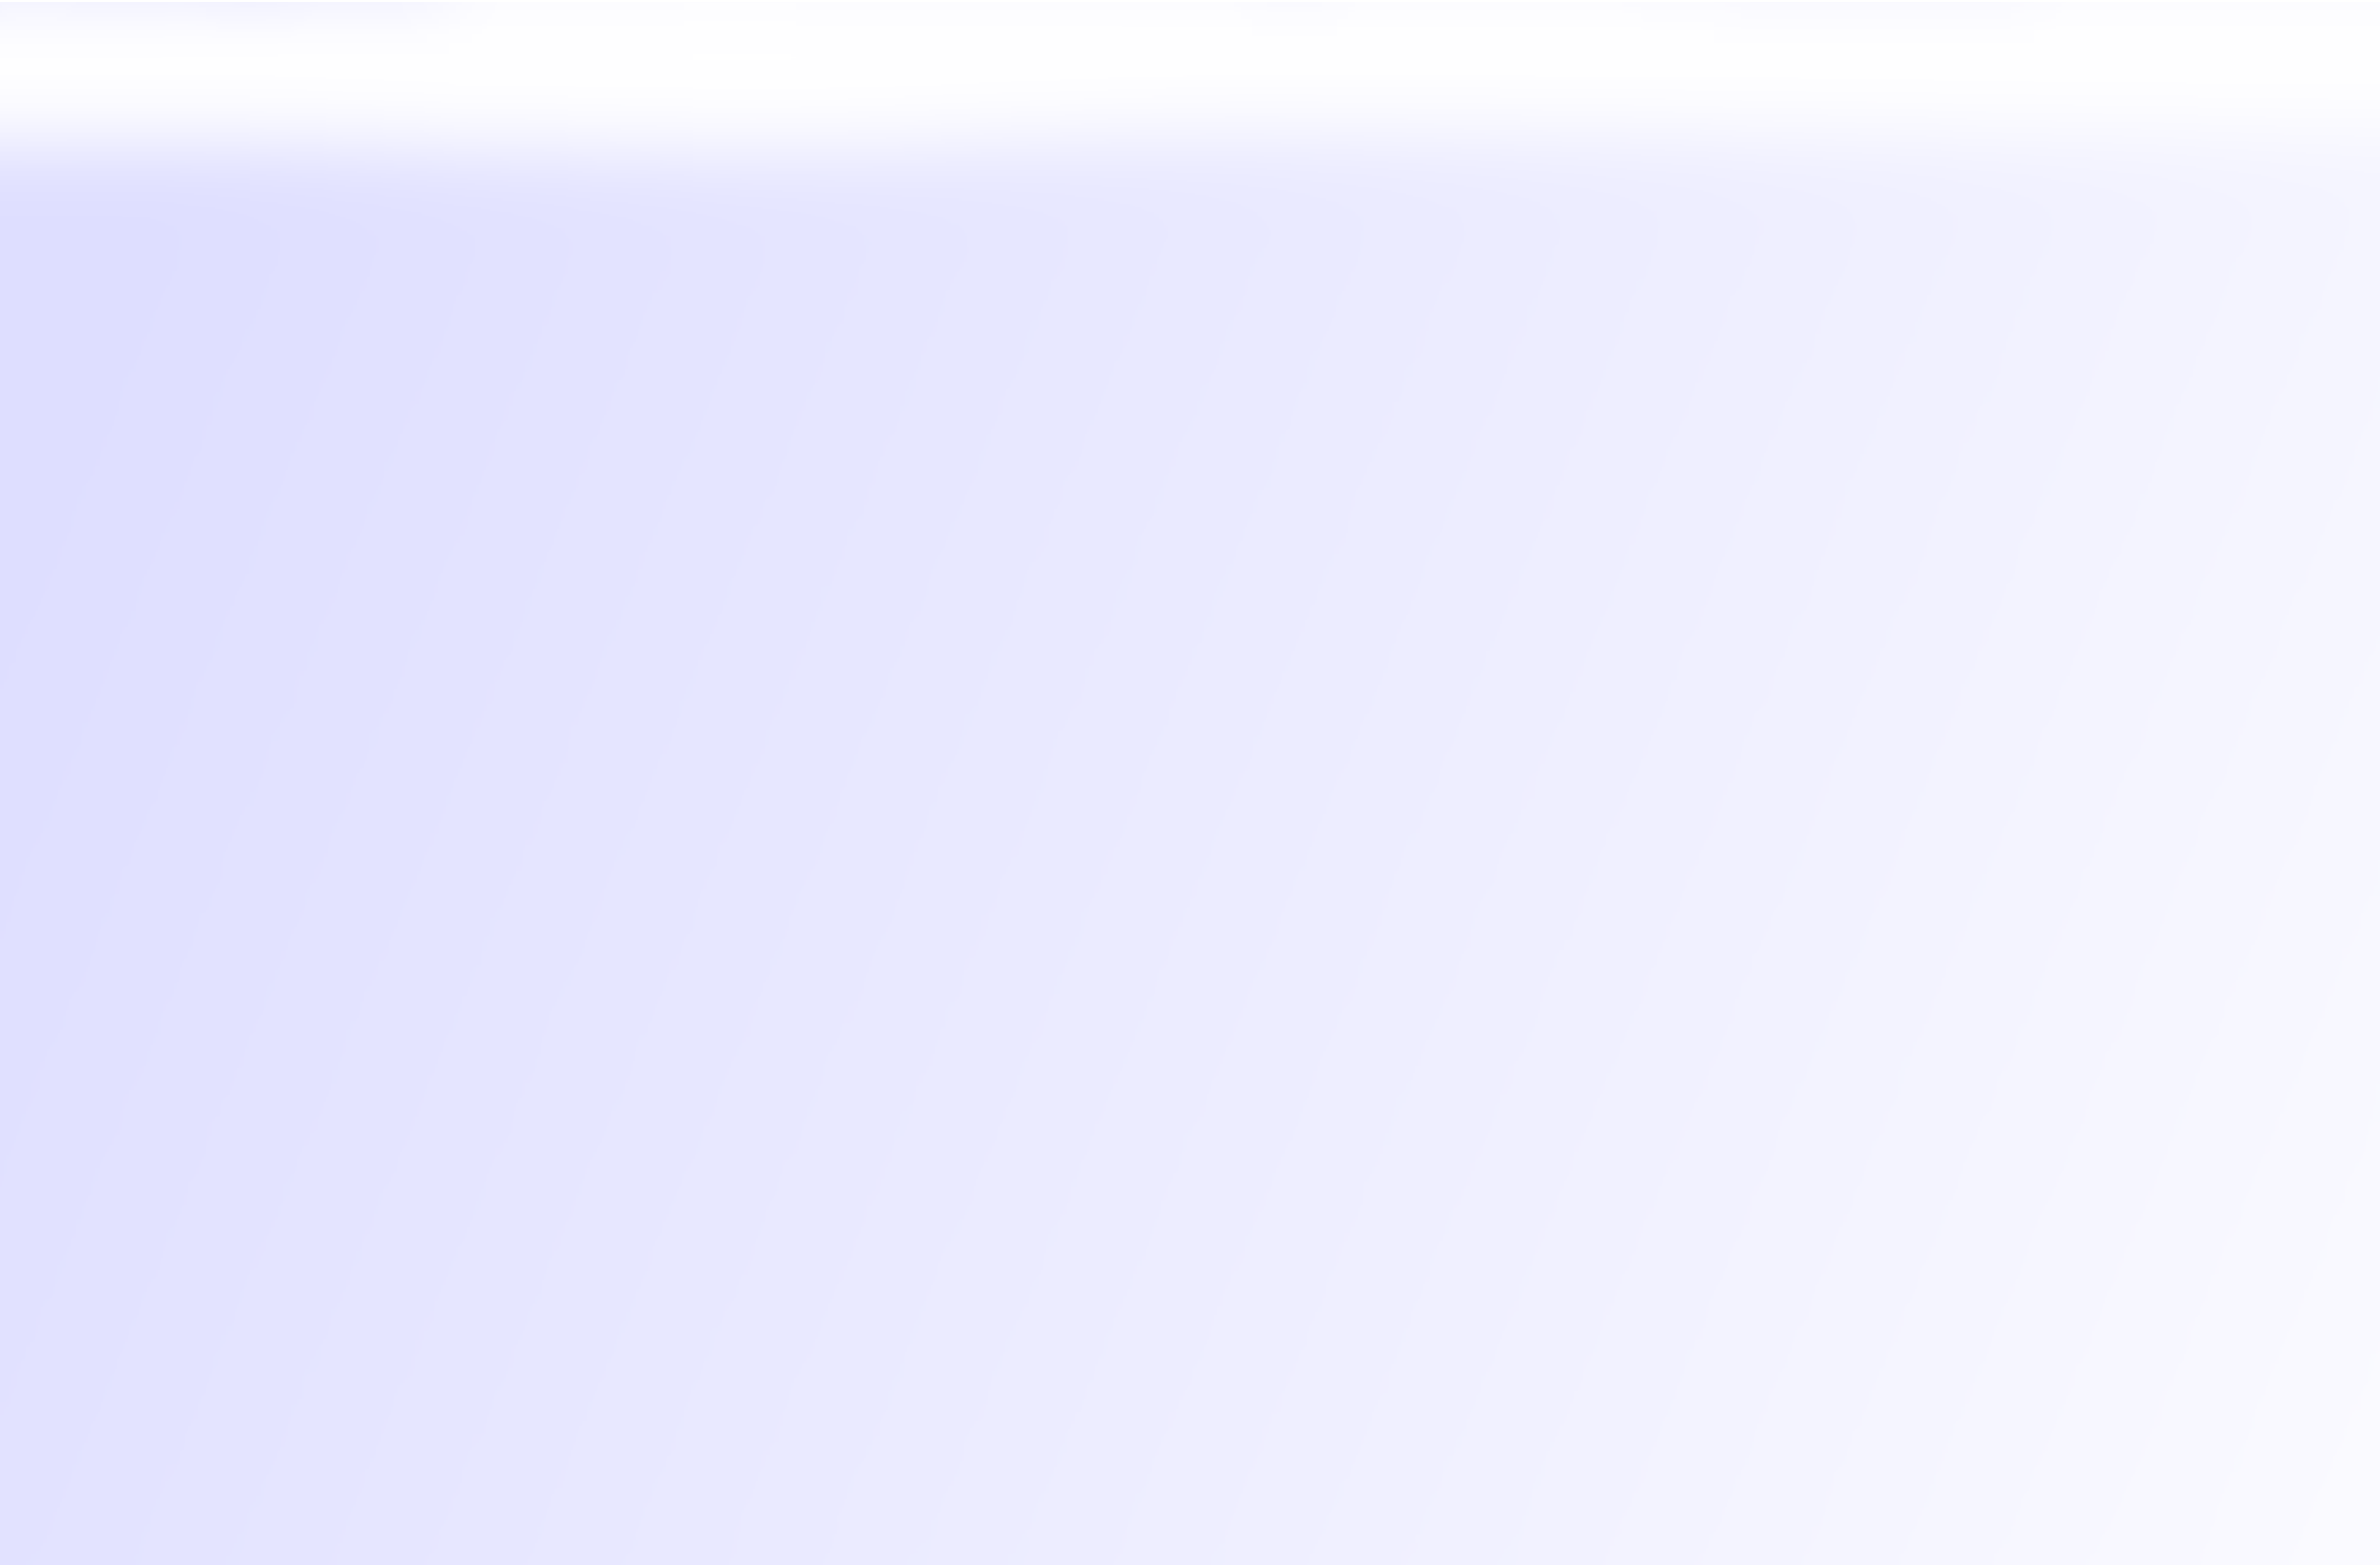
\includegraphics[height=1.1\textheight]{background}};
\end{tikzpicture}
}

\begin{poster}{
	grid=false,
	borderColor=bordercol, % Border color of content boxes
	headerColorOne=headercol1, % Background color for the header in the content boxes (left side)
	headerColorTwo=headercol2, % Background color for the header in the content boxes (right side)
	headerFontColor=headerfontcol, % Text color for the header text in the content boxes
	boxColorOne=boxcolor, % Background color for the content in the content boxes
	headershape=roundedright, % Specify the rounded corner in the content box headers
	headerfont=\Large\sf\bf, % Font modifiers for the text in the content box headers
	textborder=rectangle,
	background=user,
	headerborder=open, % Change to closed for a line under the content box headers
	boxshade=plain
}
{}
%
%----------------------------------------------------------------------------------------
%	TITLE AND AUTHOR NAME
%----------------------------------------------------------------------------------------
%
{\sf\bf Untangling the chromatin conformation \\ of the \textit{GNG12-AS1/DIRAS3} locus} % Poster title
{\vspace{0.5em} Stephen Richer, Adele Murrell, Dorothy Buck\\ 
{\vspace{0.5em} s.richer@bath.ac.uk}} 
{
\includegraphics[scale=0.8]{uob-logo.eps}}

%----------------------------------------------------------------------------------------
%	INTRODUCTION
%----------------------------------------------------------------------------------------

\headerbox{Introduction}{name=introduction,column=0, row=0}{

I study \textit{campy}. 

}

%----------------------------------------------------------------------------------------
%	MATERIALS AND METHODS
%----------------------------------------------------------------------------------------

\headerbox{Materials and Methods}{name=methods,column=0,below=introduction}{

\begin{description}
\item[ER1] Sed a orci non ipsum posuere placerat. Nunc in mi augue, a adipiscing massa. Donec dapibus gravida odio, condimentum convallis urna.\item[ER2] Nullam sagittis cursus neque, sit amet mollis elit auctor in. Etiam sed lectus a nulla rhoncus interdum a tempus nunc. Sed at eleifend purus.
\end{description}

Nullam sollicitudin lobortis urna quis varius. Nullam sagittis blandit diam, $DN = G_t(V_t,E_t)$, risus $E_t \subseteq V_t \times V_t$ ($\forall t \geq 0$). vel tortor justo, $G_0$, quis malesuada lorem.

\begin{center}
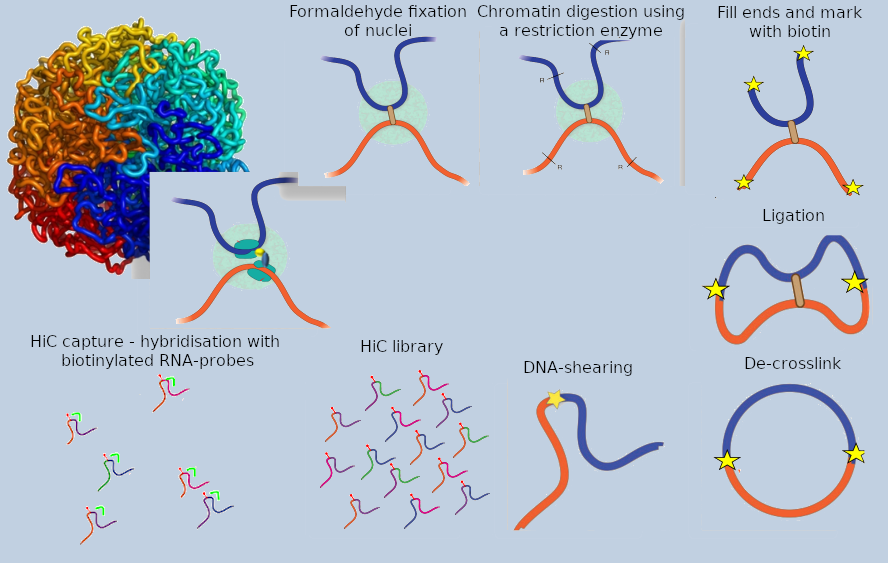
\includegraphics[width=1.0\linewidth]{hic_technique}
\captionof{figure}{Figure caption}
\end{center}

Vivamus porta lacus et lectus \textbf{porta lacus}. Pellentesque habitant morbi tristique senectus et netus et malesuada fames ac turpis. torte $G_t$ hac millis \textbf{plates} Idk 
}

%----------------------------------------------------------------------------------------
%	CONCLUSION
%----------------------------------------------------------------------------------------

\headerbox{Conclusion}{name=conclusion,column=0,below=methods}{

Fusce at erat vitae metus porttitor auctor sit amet at ante. In id dolor tellus, non aliquet elit. Vestibulum bibendum, augue sed laoreet congue, enim nisi ultricies diam, ac pharetra mi dui ut sapien. Maecenas fermentum, neque ut scelerisque consequat, purus leo ultrices nulla, quis scelerisque risus elit non turpis. 

\begin{enumerate}
\item Cras ac ipsum eu nisl imperdiet interdum nunc bibendum, est in pulvinar facilisis, mi purus fringilla tellus, eu varius ipsum ante laoreet ipsum
\item Sed cursus erat quis odio laoreet facilisis maecenas vehicula
\end{enumerate}
}

%----------------------------------------------------------------------------------------
%	REFERENCES
%----------------------------------------------------------------------------------------

\headerbox{References}{name=references,column=0,below=conclusion}{

\smaller % Reduce the font size in this block
\renewcommand{\section}[2]{\vskip 0.05em} % Get rid of the default "References" section title
\nocite{*} % Insert publications even if they are not cited in the poster

\bibliographystyle{unsrt}
\bibliography{poster} 
}

%----------------------------------------------------------------------------------------
%	RESULTS 1
%----------------------------------------------------------------------------------------

% To reduce this block to 1 column width, remove 'span=2'
\headerbox{Results Heading} {
	name = results1, span = 2, column = 1}{ 

Nunc sit amet sem ut nulla tincidunt mattis vel nec mauris. Vestibulum odio tellus, lobortis. Vel adipiscing, Aliquam dictum, ligula egestas commodo posuere, lectus lectus congue ligula, sed posuere urna lectus at nisi. Nullam varius, lacus et interdum hendrerit, odio orci ultrices mauris, id interdum eros mauris at urna. Fusce in nisi eros, sit amet volutpat turpis, \textbf{porttior magna} (commodo blandit euismod) \textbf{facilisis ornate magnis} (dis magnis). 

%------------------------------------------------
\begin{center}
\includegraphics[width=0.9\linewidth]{GNG12_AS1_DIRAS3_ontad_sum_3000_count}
\captionof{figure}{Figure caption}
\end{center}
%------------------------------------------------
}

%----------------------------------------------------------------------------------------
%	RESULTS 2
%----------------------------------------------------------------------------------------
% To reduce this block to 1 column width, remove 'span=2'
\headerbox{Chromatin conformation changes between HB2 and MCF7} {
	name = results2, span=2, column = 1, 
	below = results1, above = bottom}{

%------------------------------------------------

\begin{center}
\includegraphics[width=0.9\linewidth]{GNG12_AS1_DIRAS3_HB2_WT_vs_MCF7-logFC}
\captionof{figure}{Figure caption}
\end{center}

}

\end{poster}

\end{document}